\chapter{Metode}\label{Metode}

Dette afsnit har til formål at give et indblik i hvordan der er blevet arbejdet metodisk og videnskabeligt igennem projektet fra det initierende problem, og igennem rapporten til der opnås en endelige konklusionen. Metode kapitlet har til formål at gøre det muligt for læseren at få indsigt, hvordan vi igennem hele forløbet har arbejdet os frem til et færdigt produkt, og hvordan der overordnet er blevet arbejdet for at nå frem til dette produkt.

\section{Brainstorm og problemtræ}

Med udgangspunkt i hovede-emnet simuleringer var første proces, at undersøge mulige kategorier af under-emner, hvor man kunne se simulering som værende en del af en løsning til at afvikle et problem, samt et under-emne som et flertal synes kunne være interessant at arbejde med. Først blev gruppens medlemmer bedt at undersøge hvorvidt om det var muligt at finde noget brugbart materiale omkring de emner som de havde forslået og havde i tankerne, hvorefter de blev samlet i et problemtræ. Gruppens medlemmer fremlagde det som de havde fundet frem til, så det var muligt at vælge ved afstemning hvilket emne et flertal kunnes samles omkring til at indskrænke os.

\begin{figure}[H]
\begin{adjustbox}{width=0.75\textwidth,center=\textwidth}
\centering
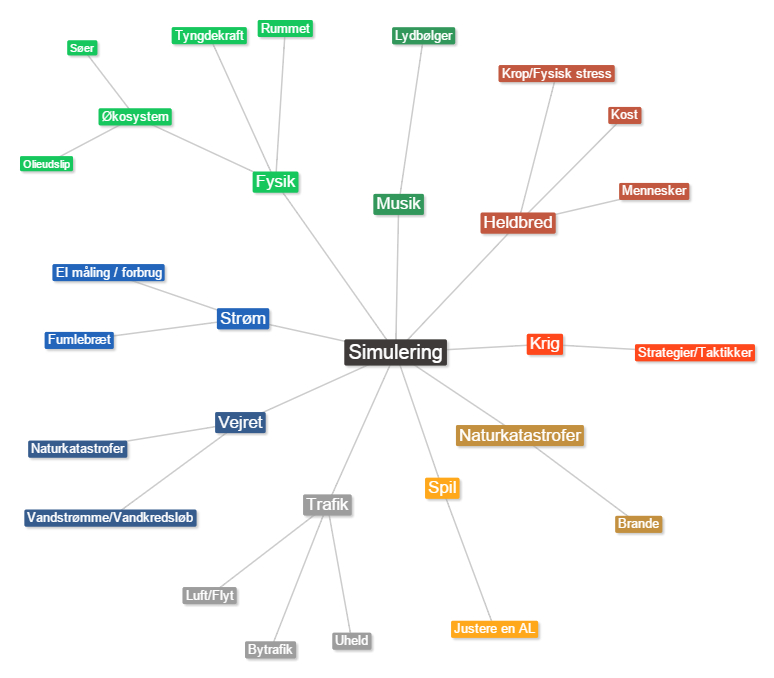
\includegraphics[width=0.75\textwidth]{Pictures/Metode/Brainstorm.jpg}
\end{adjustbox}
\label{fig:dijkstrasgraf}
\caption{Graf til fremvisning af eksempel af Dijkstras algoritme i brug}
\end{figure}

\section{Problemområde}

Fra simulering blev det besluttet at indskrænke det yderligere til trafik simulering. Efterfølgende blev samme procedure benyttet under brainstormen til at afgrænse os yderligere indenfor trafik, således at det var muligt at vælge et meget afgrænset område, hvor det var muligt at finde materiale nok at arbejde med, til at lave en udførlige problemanalyse, hvorfra det var muligt at opstille en problemformulering der kan lede videre til en problemløsning. 

\section{Fremgangsmåde}

Efter der blev gruppe

\section{Søgeprotokol}

\section{Kilder og kildekritik}

Når der blev fundet og benyttet kilder i vores projekt, blev det besluttet at alle kilder der måtte benyttes var kilder, som havde belæg i form af at det skulle være muligt at kunne kontakte vedkommende , eller have ophav fra statslige instanser eller anerkendte virksomheder og organisationer. 